\chapter[Results]{Results}
\label{sec:results}

This chapter explains the results obtained so far with the project development.


\section{Template}
\label{sec:template}

One of the goals of this work was to generate a template that allowed the game developers from the courses of this University to create their games and easily generate packages to install in major Operating Systems, namely, Windows, macOS, Debian-based and Red Hat based distributions of GNU/Linux. This template was made by professor Edson.  I had the responsibility of testing it in a few games, evolving and maintaining it throughout all the platforms.

The template consists of a series of Bash scripts, Makefile, libraries and a directory structure that is supposed to be followed by anyone who wants to use it. It is intended to be used as a template for new games developed in the courses taught at this University and it contains the most common libraries in game development, like SDL, SDL\_image, SDL\_mixer.

Currently, there are seven required files on the root directory, specifically, \texttt{LICENSE}, \texttt{Makefile.common}, \texttt{Makefile.macos}, \texttt{Makefile.windows}, \texttt{Makefile.linux}, \texttt{Vagranfile}, \texttt{changelog}, and \texttt{metadata.ini}. These files assure compilation is possible in any platform and also give some information about the project. An explanation of what each of them does and what information each may or may not have is given bellow. Some extra optional files are also explained.

\begin{itemize}
	\item \texttt{LICENSE} \emph{Editable.} This should be the text of the license or a reference to a file that has the full text. Debian packages complain if this file is the actual license text for common licenses, therefore it may be better option to only refer to a file inside the system (usually \texttt{/usr/share/common-license/LICENSE});
	\item \texttt{Makefile.macos}, \texttt{Makefile.windows}, \texttt{Makefile.linux} \emph{Uneditable.} Each of these files sets variables with specific for each system, like \texttt{CC} and \texttt{DEBUG\_FLAGS}. If a variable isn't needed 's just left blank. The template is supposed to work with values as they are and users shouldn't change them unless they \emph{actually} want a different behavior.
	\item \texttt{Makefile.common} \emph{Partially editable.} Sets some other variables, common to all OSs, like \texttt{LDFLAGS}, based on each platform Makefile. The template has set default SDL libs (SDL, SDL\_image, SDL\_mixer, SDL\_ttf), but other external libs may be wanted. When this happens, the user should add the libs wanted to the variable \texttt{EXTERNAL\_LIBS} without quotes and separated by simple space. Each of these libs must be a directory inside the \texttt{lib} folder. The rest of the file should not be changed  since it may lead to major errors when using the template, unless the user is totally sure of how it works, .
	\item \texttt{Vagranfile} \emph{Optional.} This file creates two Virtual Machines running Debian and CentOS. If the user wishes to give support for them both (generating both \texttt{.deb} and \texttt{.rpm} packages), they could either use the VMs or run the template natively on each system. The virtualization provides an easier way to do that, but it is up to the user deciding this detail of the development cycle.
	\item \texttt{changelog} \emph{Editable.} When creating the Debian package, it needs a changelog, that registers what was changed from the previous versions, much like a commit message. There are ways of generating this file automatically because its syntax is very particular, but the template doesn't contemplate it yet.
	\item \texttt{metadata.ini} \emph{Editable.} As the extension suggests, \textit{ini} stands for \textit{initialization}. This is a configuration file that follows the \texttt{ini} syntax. It defines some project properties that will be used in several steps, like building and packaging, making it a very important file to correctly use the template. The user should change this file with the appropriate information as soon as cloning the repository and throughout the development.
\end{itemize}


\section{Platform}
\label {sec:platform}

The team developing this first version of the platform was able to integrate Django and React with some difficulty. Both of the technologies chosen are very well established on their own. Putting them together, however, is another matter, where they had a real hard time to make everything work right. They used React as the main user interface and Django Admin package to create the administrator part of the game.

The website as of now allows an administrator to upload a game, with its respective information, like supported platform, related media, and installers.
The administrator has to manually add all the information related to a game, like developers who worked on it, awards won (if any), release date, version number, etc. Figure \ref{fig:include_game1} shows part of the screen to add a game.

\begin{figure}[h!]
\centering
\fbox{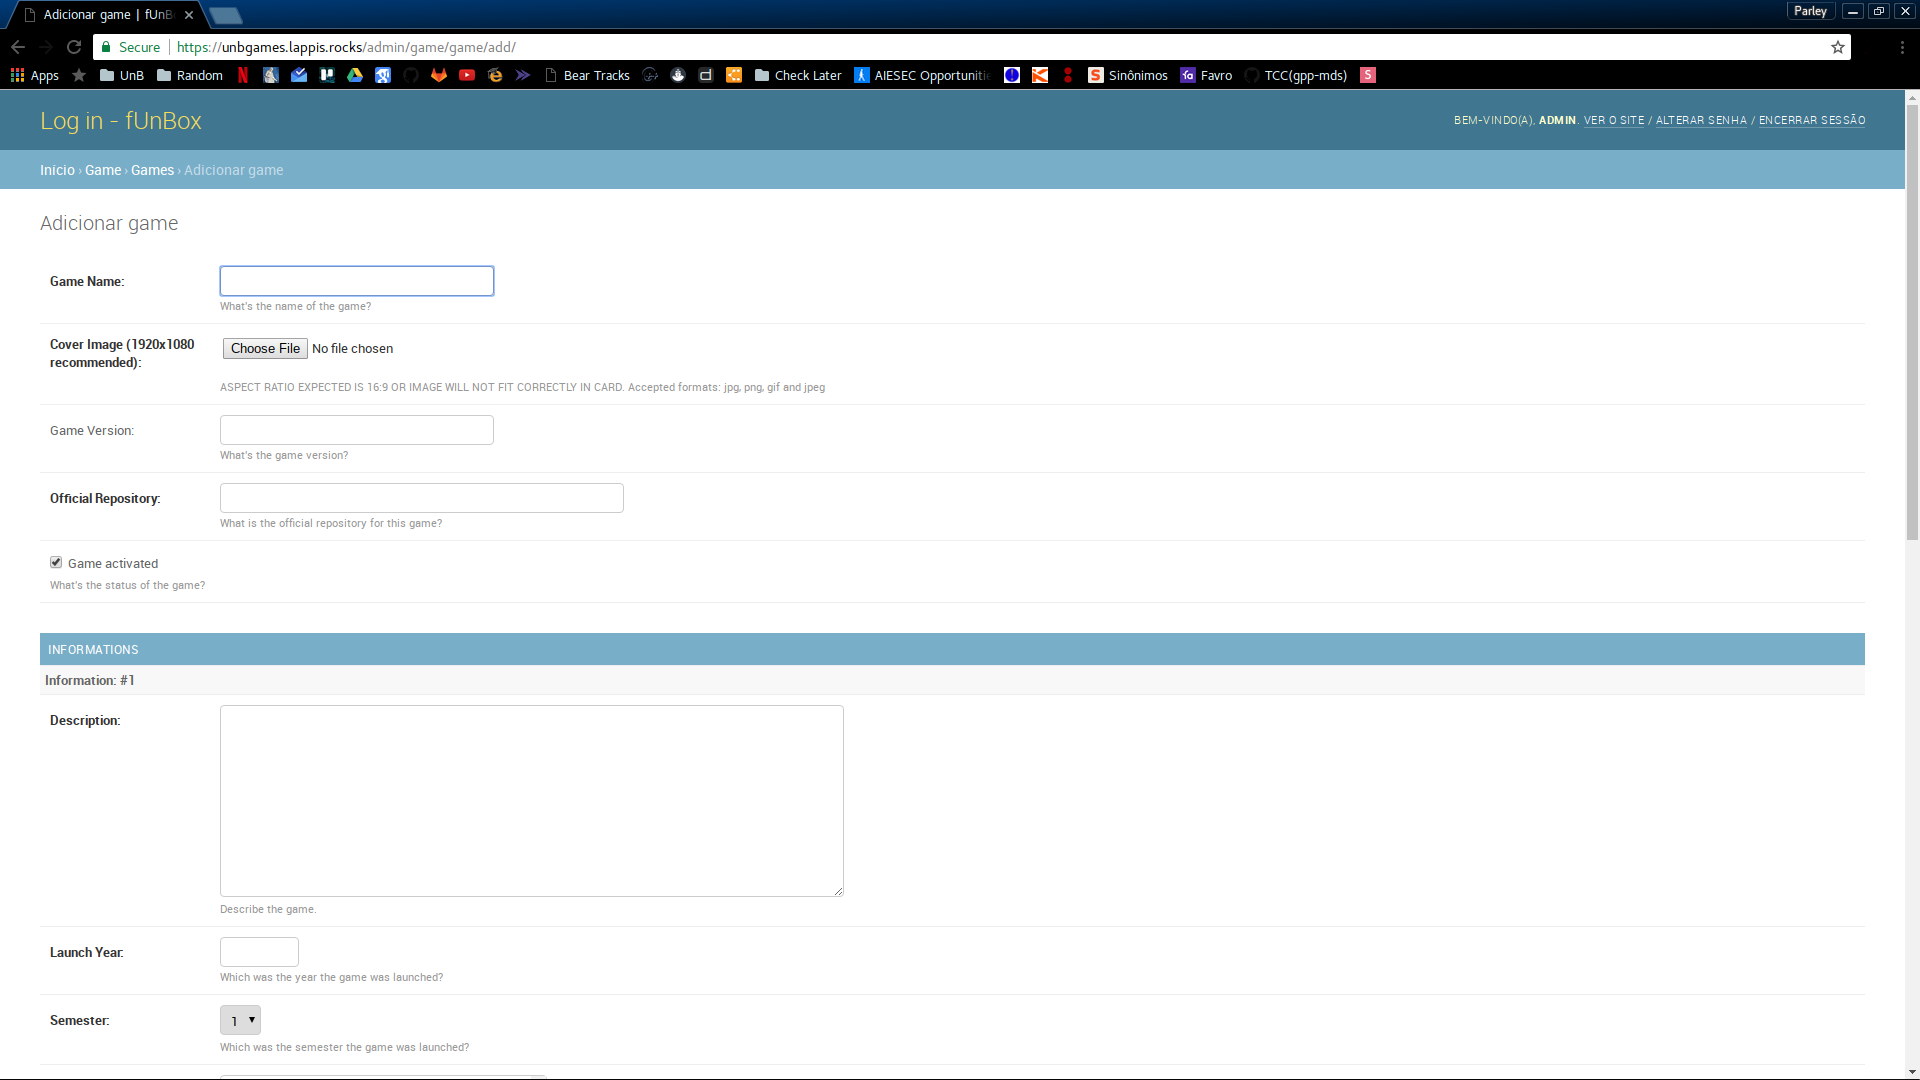
\includegraphics[width=\textwidth,height=\textheight,keepaspectratio]{include_game1}}
\caption{Include new game}
\label {fig:include_game1}
\end{figure}

The general public can see a list of the available games, with their uploaded pictures. The home page also shows a slide with some pictures of highlighted games. By choosing one, it's possible to see its version, official repository, release date, description, among other information.

Some other features of the platform are the possibility to download the game for the available operating systems or comment using a Facebook account, as shown in Figure \ref{fig:game_detail}. It's also possible to categorize the games and apply several filters to them. The user can search for a specific game by its name or description as well.

The team reported they had some problems in their inner communication on this first part of the project. They are 13 people, while 5 were the managers and 8 were developers. For people without any experience in managing and with a very detailed and demanding process, like RUP, they said it was hard to balance everything.

They also said that the transition from one process to the other was a little hard, especially the role change, holding the meetings and making sure Scrum/XP were being followed correctly. The communication problem they had in the first part was mitigated in this second part of the semester, but their main difficulty now was scoring the User Stories.

They declared that, beyond all the struggling that has been detailed above, they were too naive to choose React and Django for the development of the platform. This integration is not something very trivial for experienced programmers in both frameworks, it was even harder for developers that didn't have any experience with any of them. They said it was hard to manage everything that had to be done, learn the new technologies and still merge them together.


\begin{figure}[h!]
\centering
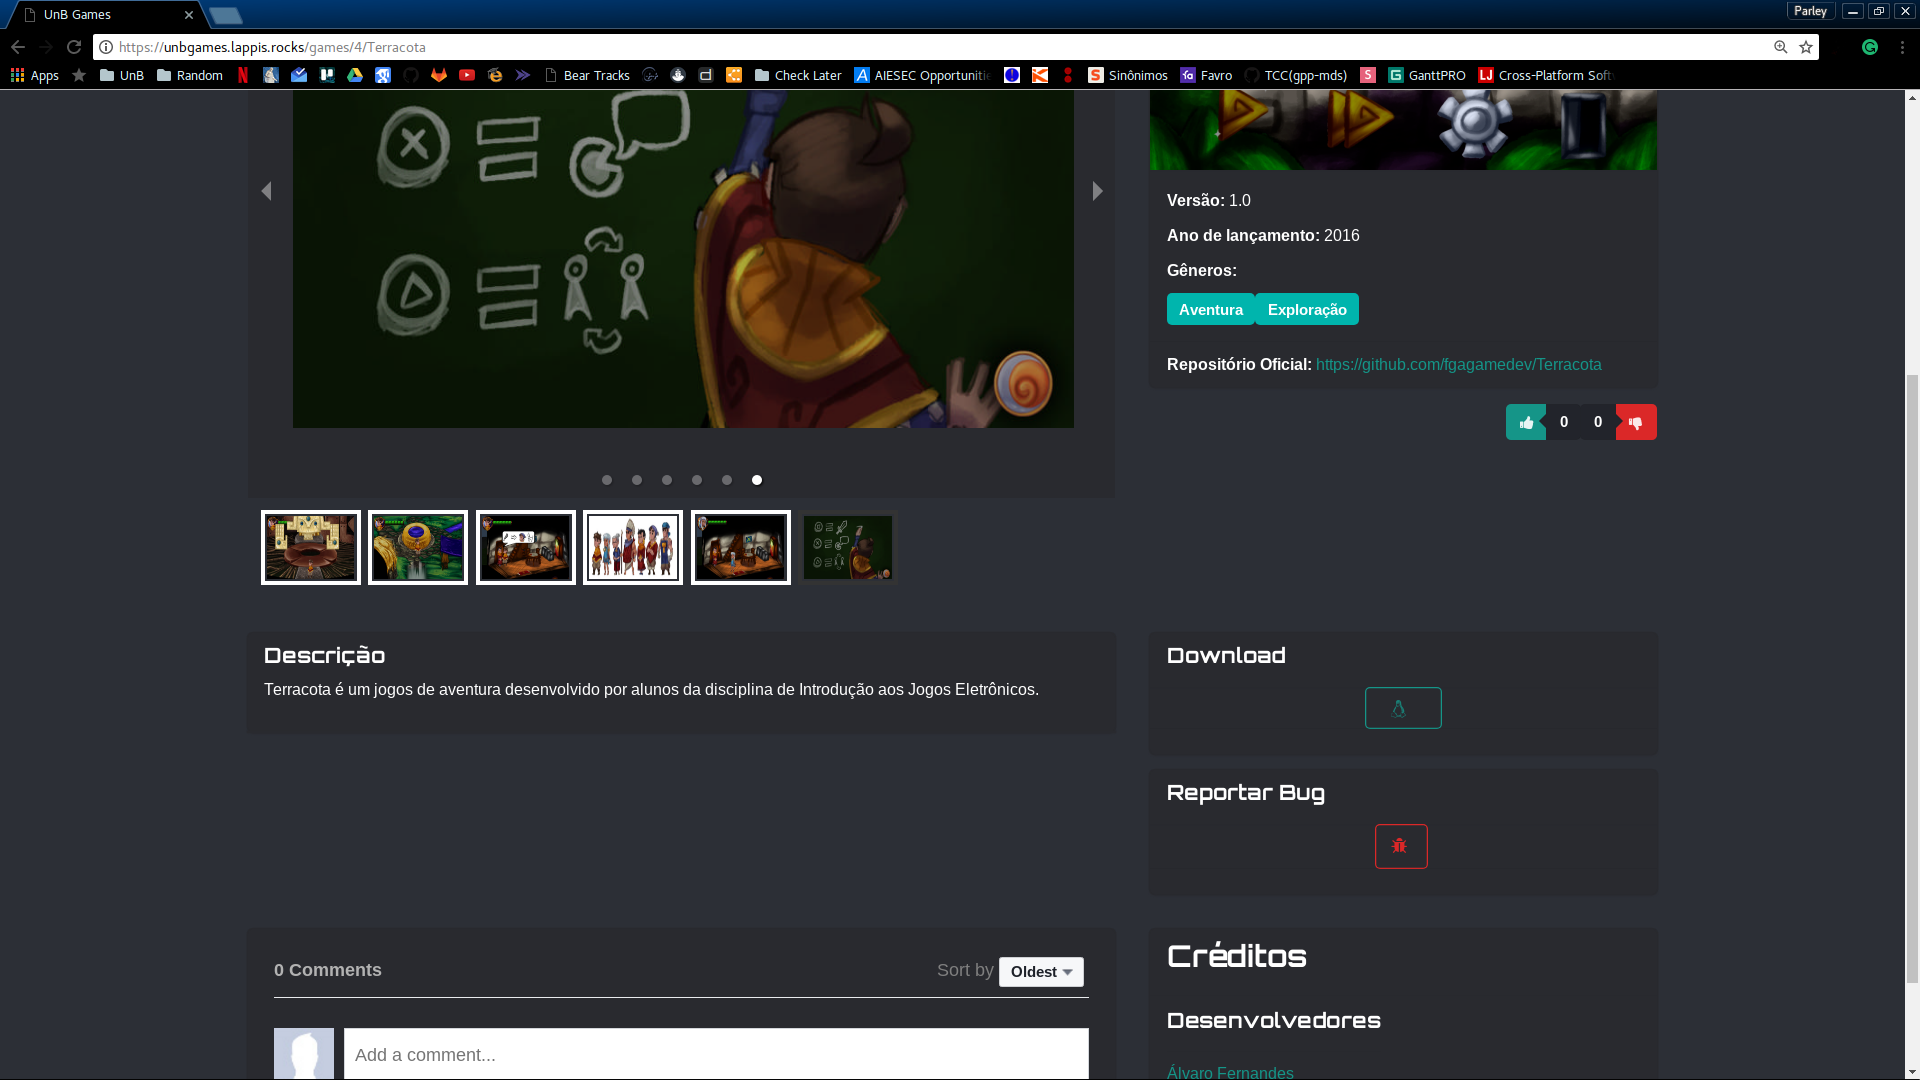
\includegraphics[width=\textwidth,height=\textheight,keepaspectratio]{terracota_detail}
\caption{Game detail}
\label {fig:game_detail}
\end{figure}

\section{Known Issues}
\label {sec:issues}

